\chapter{Probability} % (fold)
\label{cha:probability}

This chapter will focus on the main probabilistic knowledge necessary to have a
strong mathematical base. One of the key thing to know about probabilities is
that all the theory is built from the set theory. Because of that the very
first points to take into account will be the fundamental set aspects. After
that the chapter will go inside into the probabilistic theory.

\section{Set Theory} % (fold)
\label{sec:set_theory}

Informally, a set can be defined as a collection of objects. The formally
definition of what it's a set vary depending of the axiomatic definition of
choice. Because set theory is not into the aim of this book and because sets can
be studied intuitively, we are going to refer to it in his more fundamental
form. Venn diagrams can be used to understand graphically most of the properties
of sets.

\subsection{Notation}
If an object $o$ is an element of a set $A$, then we can write $o \in A$. A set
and his elements can be denoted by\didit{If you are going to put a displayed 
equation out of paragraph with comments, as in the following case, with 
\texttt{amsmath} this is the way to do it}
\begin{equation*}
    A = \{o_1, o_2, \dots , o_n\} \text{ where $n$ can be \emph{finite} or
    \emph{infinite}}
\end{equation*}

If all elements of a set $B$ are also member of a set $A$ then we can say that
$B$ is a subset of $A$ and it's denoted by $B \subset A$ or $B \subseteq A$ if
$A$ and $B$ has exactly the same elements.

Sometimes a especial set $U$ is used to refer the set that contains all possible
objects.

\subsection{Binary Operations}

Set theory defines a group of operations that can be performed between two sets.
Some of them are:\didit{This is best handled as a description list and not as a 
bullet list.}
\begin{description}
    \item \textbf{Union} of $A$ and $B$, denoted $A \cup B$, is the set of all
    objects that are a member of $A$, or $B$, or both.
    \item \textbf{Intersection} of $A$ and $B$, denoted $A \cap B$, is the set
    of all objects that are members of both $A$ and $B$.
    \item \textbf{Complement} of $A$ refers to elements not contained in $A$.
    Denoted $\overline{A}$ or $A^c$
    \item \textbf{Difference} of $A$ and $B$, denoted $A \setminus B$, is the
    set of all members of $A$ that are not members of $B$
    \item \textbf{Power} of $A$, denoted $\mathcal{P}(A)$, is the set whose
    members are all of the possible subsets of $A$. 
\end{description}

\subsection{Properties} % (fold)
\label{sub:properties}

Derived from above there is some general properties called the
\textbf{fundamental properties of set algebra}. These properties are essential
to understand the set theory. In fact, if the set theory is completely
understand, these properties are automatically assimilated. Thus it's not
necessary to memorize it. 
\begin{itemize}
   \item Commutative: \didit{A better way to insert groups of equations into a 
   document that uses \texttt{amsmath} is to use the \texttt{gather*} 
   environment as shown below}
   \begin{gather*}
        A \cup B = B \cup A\\
        A \cap B = B \cap A     
   \end{gather*}
   \item Associative: 
   \begin{gather*}
        (A \cup B) \cup C = A \cup (B \cup C)\\
        (A \cap B) \cap C = A \cap (B \cap C)        
   \end{gather*}
   \item Distributive:
   \begin{equation*}
        \text{Union with Intersection:} \quad 
        \begin{gathered}
            (A \cap B)\cup C = (A\cup C) \cap (B \cup C)
        \end{gathered}
    \end{equation*}
    \begin{equation*}
        \text{Intersection with Union:} \quad
        \begin{gathered}
             (A \cup B)\cap C = (A\cap C) \cup (B \cup C)
         \end{gathered}
   \end{equation*}   
   \item Neutral Element: $A \cup \emptyset = A = A \cap S$
   \item Complementation: $A \cup \overline{A} = S$ and $A\cap \overline{A} =
   \emptyset$
   \item Idempotence: $A \cup A = A$ and $A \cap A = A$
   \item Abosortion: $A \cup S = S$ and $A \cap \emptyset = \emptyset$
   \item Simplication: $A \cap (A \cup B) = A = A \cup (A \cap B)$
\end{itemize}

\minisec{De Morgan's laws}

\todo[inline,color=red!40]{Instead of marking with boldface a header that 
lacks meaning within the structure of the document, it' s better to use the 
minisec instruction that KOMA Script gives us when we want to put a header 
without numbering or appearing in the table of contents.}

\begin{gather*}
   \overline{A \cup B} = \overline{A} \cap \overline{B}
   \overline{A \cap B} = \overline{A} \cup \overline{B}
\end{gather*}
% subsection properties (end)
% section set_theory (end)

\section{Combinatory} % (fold)
\label{sec:combinatory}

Also know as expertise in counting

\subsection{Rule of Product} % (fold)
\label{sub:rule_of_product}

If there are $\alpha$ ways of doing something and $\beta$ ways of doing another
thing, then there are $\alpha\beta$ ways of performing both actions.
% subsection rule_of_product (end)

\subsection{k-permutations} % (fold)
\label{sub:k_permutations}

\minisec{k-permutations of n elements:}

The number of \textbf{ordered sequences} with $1\leq k \leq n$ that can be
formed of $n$ elements is,
\begin{equation*}
n(n-1)(n-2)\dots(n-k+1) = \dfrac{n!}{(n-k)!}
\end{equation*}
% subsection k_permutations (end)

\subsection{k-combinations} % (fold)
\label{sub:k_combinations}

\minisec{k-combinations of n objects:}

The number of \textbf{unordered sequences} within a set with $1\leq k \leq n$
that can be formed of $n$ elements is,
\begin{equation*}
\binom{n}{k} = \dfrac{n!}{k!(n-k)!}
\end{equation*}
% subsection k_combinations (end)

\subsection{Partitions} % (fold)
\label{sub:partitions}

$r$ groups containing $n_i$ objects each,
\begin{equation*}
\binom{n}{n_1,n_2\dots,n_r} = \dfrac{n!}{n_1!n_2!\dots n_r!}
\end{equation*}
% subsection partitions (end)
% section combinatory (end)

\section{Random Experiments} % (fold)
\label{sec:random_experiments}

 A experiment is deterministic when knowing the state of the set of variables
 involved in the experiment the outcome is always the same. Conversely a
 experiment is random when knowing the state (or when we ignore some of these
 states) of the set of variables involved in the experiment the outcome differs.
 
 In other terms, \textbf{an experiment is random} if although it is repeated in
 the same manner every time, can result in different outcomes. Thus, the fixed
 outcome of a random experiment is impossible to predict in advance although the
 number of individual possibles outcomes is known in advance. The probability
 theory study the random experiments.\didit{To separate paragraphs, just leave a 
 blank line between them. It isn't necessary to use the double backslash for it, 
 on the contrary it overloads the compiler and can generate unexpected errors.}

 The notation of some elements involved in a random experiment are the
 followings:
 \begin{description}
     \item[Sample Space,] is the set of all possible outcomes of the
     random experiment. It's denoted by $S$ or $\Omega$
     \item[Individual Outcomes,] are the type of possible outcomes of a
     random experiment. It's denoted by $\omega$
     \item[Event,] is a subset of $S$. Usually denoted by capital
        letters starting by $A$, $B$, $C$, etc. Sometimes denoted by
        $\mathcal{F}$ for his general form. 
     \item[Null Event,] is a special event that never occurs. Denoted by
     $\emptyset$
     \item[Frequency,] of $\omega$ is the number of times the individual
     outcome $\omega$ occurs in a random experiment.
     \item[Relative Frequency] of $\omega$ is the ratio between the
     frequency of $\omega$ and the total number of outcomes of a random
     experiment.
 \end{description}

 Once the experiment has been performed, it is said that $A$ \enquote{happened} if the
 outcome of the experiment ($\omega$) belongs to $A$. 

\subsection{Events Operations} % (fold)
\label{sub:events_operations}

If the logical meaning from the set operations is taken and restricted to a
probabilistic perspective, then a new meaning for these operations can be
defined in this new scope. Thus:
\begin{description}
    \item[Union] $A \cup B$ (Grammatically $A$ or $B$), occurs when
    either of the two events (or both of them simultaneously) do occur.
    \item[Intersection] $A \cap B$ (Grammatically $A$ and $B$), occurs
    when both of them do simultaneously occur.
    \item[Complementary] $\overline{A}$ (Grammatically not $A$), occurs
    when the event does not occur.
    \item[Difference] $A \setminus B$ (Grammatically $A$ and not $B$),
    occurs when the first event does occurs, but the second does
    not. Note that $A \setminus B = A \cap \overline{B}$
\end{description}
% subsection events_operations (end)

\subsection{Formal Definitions} % (fold)
\label{sub:formal_definitions}

From an formal perspective, the concept of probability has been defined
multiples times. Here they are collected the fundamental ones that tries to
formalize the abstract concepts of what it's usually understand as probability
and his parts.

\subsubsection{$\sigma$-algebra} % (fold)
\label{ssub:_sigma_algebra}

A $\sigma$-algebra (sigma-algebra) $\mathcal{A}$ over a set $\Omega$ is a family
(collection) of subsets (with elements $E_1, E_2, \dots$) of $\Omega$ that
satisfies:
\begin{itemize}
    \item $\emptyset \in \mathcal{A}$
    \item If $E \in \mathcal{A}$ then $\overline{E} \in \mathcal{A}$
    \item If $E_1, E_2, \dots \in \mathcal{A}$ then $\cup_{n=1}^{\infty}E_i \in
    \mathcal{A}$ 
\end{itemize} 
% subsubsection _sigma_algebra (end)

\subsubsection{$\sigma$-algebra discrete} % (fold)
\label{ssub:_sigma_algebra_discrete}

The discrete $\sigma$-algebra of $\Omega$ is the power set of $\Omega$
($\mathcal{P}(\Omega)=\{E : E \subset \Omega\}$), that is, the collection of all
subsets of $\Omega$.\\

\textbf{For example,} given a random experiment that toss one coin,
\begin{description}
    \item[$H$:] The coin shows head.
    \item[$T$:] The coin shows tail. 
    \item[$S =$] $\{H, T\},\;\;\; \mathcal{P}(S)=\{\emptyset, \{H\}, \{T\}, S\}$
\end{description}
% subsubsection _sigma_algebra_discrete (end)

\subsubsection{Measurable Space} % (fold)
\label{ssub:measurable_space}

The pair $(\Omega, \mathcal{A})$ is a measurable space if $\mathcal{A}$ is a
$\sigma$-algebra over $\Omega$
% subsubsection measurable_space (end)

\subsubsection{Frequentist Definition} % (fold)
\label{ssub:frequentist_definition}

The probability of an event $A$ is the limit of the relative frequency of that
event when the number of repetitions of the experiment tends to infinity. If the
experiment is repeated $n$ times, and $n_A$ is the number of repetitions in
which $A$ happens, then the probability of $A$ is
\begin{equation*}
    P(A) = \lim_{n \rightarrow \infty} \dfrac{n_A}{n}
\end{equation*}
% subsubsection frequentist_definition (end)

\subsubsection{Laplace's Definition} % (fold)
\label{ssub:laplace_s_definition}

This definition can be used for random experiments that have a finite number of
outcomes and all of them are equally likely.

The probability of an event $A$ is the ratio between the favorable outcomes to
$A$ and the total outcomes of the experiment, thus,
\begin{equation*}
    P(A) = \dfrac{\#A}{\#\Omega}
\end{equation*}

This implies that, given,
\begin{equation*}
    S = \{s_1,s_2,\dots\, s_n\},\;\;\; P(s_n)=\dfrac{1}{n}
\end{equation*}
% subsubsection laplace_s_definition (end)

\subsubsection{Kolmogorov's Definition} % (fold)
\label{ssub:kolmogorov_definition}

The Kolmogorov's definition is the only one that does not define what is a
probability function. In fact, this definition establish three axioms that must
be satisfied by any probability function. This axioms are a fundamental part of
probability theory.

Let the pair $(\Omega, \mathcal{A})$ be a \emph{measurable space}. In it, the
probability function $P$ of some event $E$, denoted $P(E)$ is an application
over the real numbers ($P: \mathcal{A} \rightarrow \mathbb{R}$) that satisfies:

\begin{description}
    \item[Non Negativity:] $P(E) \geq 0, \forall E \in \mathcal{A}$
    \item[Unitarity:] $P(\Omega) = 1$
    \item[Additivity:] Any countable sequence $E_1, E_2, \dots$ of
    disjoint events of $\mathcal{A}$, satisfies
    \begin{equation*}
        P\Bigl(\bigcup_{n=1} E_i \Bigr) = \sum_{n=1} P(E_i)
    \end{equation*}
\end{description}
% subsubsection kolmogorov_definition (end)

\subsubsection{Cox's Theorem} % (fold)
\label{ssub:cox_s_theorem}

Used by bayesians. \todo{write explanation}

% subsubsection cox_s_theorem (end)
% subsection formal_definitions (end)

\subsection{Properties} % (fold)
\label{sub:properties}

These are the properties that apply independence of the probability definition
of choice.
\begin{itemize}
    \item $P(\overline{A}) = 1 - P(A)$
    \item $P(\emptyset) = 0$
    \item If $A \subseteq B$ then $P(A) \leq P(B)$
    \item $P(A\setminus B) = P(A) - P(A \cap B)$
    \item $P(A \cup B) = P(A) + P(B) - P(A \cap B)$
    \item $P(A \cup B \cup C) = P(A \cup (B \cup C)) = P(A) + P(B) + P(C) +
    P(A\cap B \cap C) - P(A \cap B) - P(A \cap C) - P(B \cap C)$
\end{itemize}
% subsection properties (end)

\subsection{Conditional Probability} % (fold)
\label{sub:conditional_probability}

The probability of the event $A$ occurs knowing before hand that the event $B$
has occurred is,
\begin{equation*}
    P(A|B) = \dfrac{P(A\cap B)}{P(B)}
\end{equation*}

Note that when we have a conditional probability, it can be say that $B$ becomes
 the new sample space of the experiment.

\subsubsection{Properties} % (fold)
\label{ssub:properties}

The conditional probability holds all the properties of the regular probability.

% subsubsection properties (end)
% subsection conditional_probability (end)

\subsection{Bayes Theorem} % (fold)
\label{sub:bayes_theorem}

Given a set of events $A_1, A_2, \dots, A_n$, the probability of all of them
occurring simultaneously is called \textbf{probability chain rule}, and it is
\didit{When we have very long expressions it' s better to divide them instead 
of exceeding the width of the text box as follows}
\begin{equation*}
    \begin{split}
        P(A_1\cap A_2 \cap \dots \cap A_n) &= P(A_1)P(A_2|A_1)\dots P(A_n|A_1\cap \dots \cap A_{n-1})\\
                                           &= \prod_{k=1}^{n}P\Bigl(A_k|\bigcap_{j=1}^{k-1}A_j\Bigr)
    \end{split}
\end{equation*} 
or alternatively, in its two-event form,
\begin{equation*}
    P(A \cap B) = P(A)P(B|A)
\end{equation*}

\subsubsection{Total Probability Rule} % (fold)
\label{ssub:total_probability_rule}

Given $A_1,\dots,A_n$ mutually exclusive (disjoint) events whose union is the
whole of the sample space (partition) and assume $P(A_i) > 0$ for every $i$ .For
every event $B$ we have\didit{In addition to dividing long expressions it is 
convenient to use the right size brackets when using large operators.}
\begin{equation*}
    \begin{split}
        P(B) &= P(A_1\cap B) + \dots + P(A_n \cap B)\\
             &= \prod_{k=1}^{n}P\Bigl(A_k|\bigcap_{j=1}^{k-1}A_j\Bigr)
    \end{split}
\end{equation*}
% subsubsection total_probability_rule (end)

\subsubsection{Bayes Theorem} % (fold)
\label{ssub:bayes_theorem}

Knowing of above, then we can write,
\begin{equation*}
    \begin{split}
        P(A|B) &= \dfrac{P(A)P(B|A)}{P(B)}\\
               &= \dfrac{P(A)P(B|A)}{P(A_1\cap B) + \dots + P(A_n \cap B)}
    \end{split}
\end{equation*}
% subsubsection bayes_theorem (end)
% subsection bayes_theorem (end)

\subsection{Independence of two events} % (fold)
\label{sub:independence_of_two_events}

Two events are independence if and only if,
\begin{equation*}
    P(A\cap B) = P(A)P(B)
\end{equation*}

If $A$ and $B$ are independent, then the occurrence of $A$ does not provide any
information about $B$. Formally,
\begin{tcolorbox}
    If $A, B$ are independent and $P(B)>0$ then
    \begin{equation*}
        P(A|B) = \dfrac{P(A\cap B)}{P(B)} =
    \dfrac{P(A)\cancel{P(B)}}{\cancel{P(B)}} = P(A)
    \end{equation*}
\end{tcolorbox}

\subsubsection{Conditional Independence} % (fold)
\label{ssub:conditional_independence}

Given two events $A$ and $B$, they are conditionally independence if given $C$
and $P(C)>0$, \didit{When we have to interrupt the display of equations with 
text, it can be solved in the following way}
\begin{gather*}
    P(A\cap B|C) = P(A\cap C|B\cap C)
    \intertext{and}
    P(A|B\cap C) = P(A|C)
\end{gather*}

\missingfigure{explanatory Venn diagram}
% subsubsection conditional_independence (end)
% subsection independence_of_two_events (end) 
% section random_experiments (end)

\section{Discrete Random Variables} % (fold)
\label{sec:discrete_random_variables}

When we are dealing with random experiments, it's very common to use a number to
represent a event of the sample space. It's called random variable.

A \textbf{random variable} (r.v.) is the numerical outcome of a random
experiment. Formally, a random variable $X$ is a mapping $X: \Omega \rightarrow
\mathbb{R}$ \todo{Write formal definition using Borel sigma-algebra}

It associates each outcome of a random experiment with a real number and is
measurable because the inverse image of every borelian set does belong to the
$\sigma$-algebra of events.\todo{It is necessary to insert a subsection or 
level up the subsequent subsubsection}

\subsubsection{Support of Random Variables} % (fold)
\label{ssub:support_of_random_variables}

We can define the support of the random variable depending of the size of the
mapped set. A r.v. is:
\begin{description}
    \item[Discrete] if $X(\Omega)$ is a finite or numerable set.
    \item[Continuous] if $X(\Omega)$ contains an interval of
    $\mathbb{R}$
\end{description}
% subsubsection support_of_random_variables (end)

\subsection{Probability Mass Function} % (fold)
\label{sub:probability_mass_function}

A probability mass function (p.m.f.) match a real number $x$ with the
probability that an event exactly occurs.
\begin{equation*}
    p(x)=P(X=x)=P_X(x), \quad\forall x\in \mathbb{R}
\end{equation*}

% \includegraphics[width=2cm, height=1cm]{random_variables_1}

\subsubsection{Properties} % (fold)
\label{ssub:properties01}

\todo[inline]{write this}
% subsubsection properties01 (end)
% subsection probability_mass_function (end)

\subsection{Cumulative Distribution Function} % (fold)
\label{sub:cumulative_distribution_function}

The cumulative distribution function (c.d.f.) measures the probability that an
event is not greater or equal than a real number.
\begin{equation*}
    F(x) = P(X\leq x) = P_X((-\infty,x])), \quad\forall x \in \mathbb{R}
\end{equation*}

\subsubsection{Properties} % (fold)
\label{ssub:properties02}

% subsubsection properties02 (end)

\begin{itemize}
    \item $\lim_{x \rightarrow -\infty} F(X) = 0$
    \item $\lim_{x \rightarrow \infty} F(X) = 1$
    \item $F$ is non-decreasing
    \item $F$ is right-continuous
\end{itemize}
% subsection cumulative_distribution_function (end)

\subsection{Mean, Variance and Standard Deviation} % (fold)
\label{sub:mean_variance_and_standard_deviation}

\subsubsection{Mean or Expectation} % (fold)
\label{ssub:mean_or_expectation}

Let $X$ be a r.v. with the probability function $p(x)$, then, the
\emph{expected value} of $X$ is,
\begin{equation*}
    \mu_{X} \approx \mathbb{E}[X] = \sum_{x} x\,P(X=x)
\end{equation*}
if $p(x)$ is an accurate characterization of the \emph{population} frequency
distribution, then,
\begin{equation*}
    \mu_{X} = \mathbb{E}[X].
\end{equation*}
% subsubsection mean_or_expectation (end)

\subsubsection{Properties} % (fold)
\label{ssub:properties03}

\begin{itemize}
    \item $\mathbb{E}[c] = c$, if $c$ is a constant
    \item $\mathbb{E}[aX+b]= a\mathbb{E}[X]+b$
    \item $\mathbb{E}[g(x)]= \sum_{x}g(x)P(X=x)$
    \item $\mathbb{E}[X^k] = \sum_{x} x^k P(X=x)$
    \item $\mathbb{E}[X+Y] = \mathbb{E}[X] + \mathbb{E}[Y]$
    \item $\mathbb{E}[X-Y] = \mathbb{E}[X] - \mathbb{E}[Y]$
    \item $\mathbb{E}[XY] = \mathbb{E}[X]\mathbb{E}[Y]$, if $X$ and $Y$ are
    independent
\end{itemize}
% subsubsection properties03 (end)

\subsubsection{Variance} % (fold)
\label{ssub:variance}

Let $X$ be a r.v. with mean $\mathbb{E}[X] = \mu$, probability function $p(x)$,
then, the variance of $X$ is defined to be the expected value of $(X-\mu)^2$,
thus,
\begin{equation*}
    \begin{split}
        \sigma^2_X \approx V[X] &= \mathbb{E}[(X-\mu)^2] \\
                                &= \mathbb{E}[X^2] - \mu^2 \\
                                &=\sum_{x}(x-\mathbb{E}[X])^2 P(X=x)
    \end{split}
\end{equation*}
if $p(x)$ is an accurate characterization of the \emph{population} frequency
distribution, then,
\begin{equation*}
    \sigma^2_{X} = V[X]
\end{equation*}
% subsubsection variance (end)

\subsubsection{Properties} % (fold)
\label{ssub:properties04}

\begin{itemize}
    \item $V[X] \geq 0$
    \item $V[aX + b] = a^2V[X], \;\;\; \forall a,b \in \mathbb{R}$
    \item $V[X \pm Y] = V[X] + V[Y]$, if $X$ and $Y$ are independent.
    \item $V[X + Y] = V[X] + V[Y] + 2 \Cov(X,Y)$
\end{itemize}
% subsubsection properties04 (end)

\subsubsection{Standard Deviation} % (fold)
\label{ssub:standard_deviation}

The standard deviation of $X$, is the positive square root of $V[X]$
\begin{equation*}
    \sigma = \sqrt{V[X]}
\end{equation*}
% subsubsection standard_deviation (end)
% subsection mean_variance_and_standard_deviation (end)

\subsection{Median and Quantiles} % (fold)
\label{sub:median_and_quantiles}

\subsubsection{Median} % (fold)
\label{ssub:median}

The median is the most central value of a distribution of a r.v. $X$, thus, the
median $m$ of $X$ satisfies,
\begin{gather*}
    P(X \leq m) \geq \dfrac{1}{2}\\
    \intertext{and}
    P(X \leq m) \leq \dfrac{1}{2}
\end{gather*}

\missingfigure{explanatory image}
% subsubsection median (end)

\subsubsection{$\alpha$-quantiles} % (fold)
\label{ssub:_alpha_quantiles}

For $0 < \alpha < 1$ the $\alpha$-quantile of a r.v. $X$ is a number $q_\alpha$
that satisfies,
\begin{gather*}
    P(X \leq q_\alpha) \geq \alpha\\
    \intertext{and}
    P(X \geq q_\alpha) \geq 1- \alpha
\end{gather*}

\missingfigure{explanatory image}

% subsubsection _alpha_quantiles (end)
% subsection median_and_quantiles (end)

\subsection{Quantile Function} % (fold)
\label{sub:quantile_function}

For $0 < \alpha < 1$ the \emph{quantile function} of a r.v. is defined as,
\begin{equation*}
    F^{-1}_X (\alpha) = \inf \{ x : F(x) \geq \alpha 
\end{equation*}

\missingfigure{explanatory image}

\subsubsection{Properties} % (fold)
\label{ssub:properties05}

\todo[inline]{write this}

% subsubsection properties05 (end)
% subsection quantile_function (end)
% section discrete_random_variables (end)

\section{Discrete Random Distributions} % (fold)
\label{sec:discrete_random_distributions}

\subsection{Bernoulli Process} % (fold)
\label{sub:bernoulli_process}

A \textbf{Bernoulli process} is random experiment in which outcome can only
result in two different values. This outcomes are commonly referred as
\emph{success} and \emph{failure}. The probability of success is $0 \leq p
\leq 1$ and all experiment trials are \emph{independent}.
\begin{equation*}
    X \sim Bernoulli(p)
\end{equation*}
% subsection bernoulli_process (end)

\subsection{Binomial Distribution} % (fold)
\label{sub:binomial_distribution}

Consider a Bernoulli process with probability of success $p$ and that is carried
out independently $n$ times, a Binomial random variable $X$ with parameters $n$
and $p$ represents the number of trials that result in success.
\begin{gather*}
    X \sim B(n, p)\\
    \intertext{with}
    P(X=x) = \binom{n}{x}p^x(1-p)^{n-x}, \quad x \in \{0,1,2,\dots,n\}\\
    \intertext{and have expectation and variance}
    \E[X] = np, \quad V[X] = np(1-p)
\end{gather*}

\textbf{Note: Be careful with the definition.} It's not the same \enquote*{number of
trials} and \enquote{number of success}.\todo{Add base example that serves as base
 experiment.} 

Using this base experiment we cant try to fit other rand. exp. and see if this 
distribution is valid.
% subsection binomial_distribution (end)

\subsubsection{Properties} % (fold)
\label{ssub:properties06}

If $X$ and $Y$ are independent, and $X \sim B(n_1, p), Y \sim B(n_2, p)$ then 
\begin{equation*}
    X+Y \sim B(n_1+n_2, p)
\end{equation*}

\begin{figure}[!ht]
    \begin{minipage}{0.45\linewidth}
      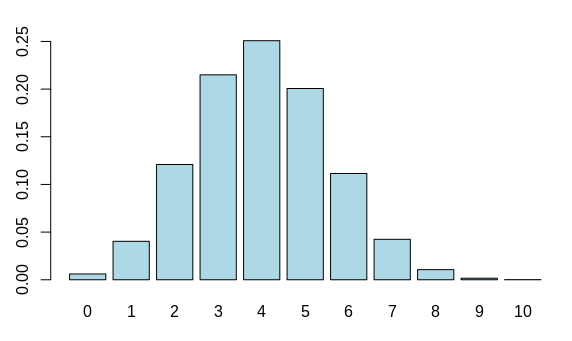
\includegraphics[width=0.99\linewidth]{random_distribution_binomial_1}
      \caption{Binomial p.m.f.}
      \label{fig:bin_pmf}
    \end{minipage}
    \hfill
    \begin{minipage}{0.45\linewidth}
      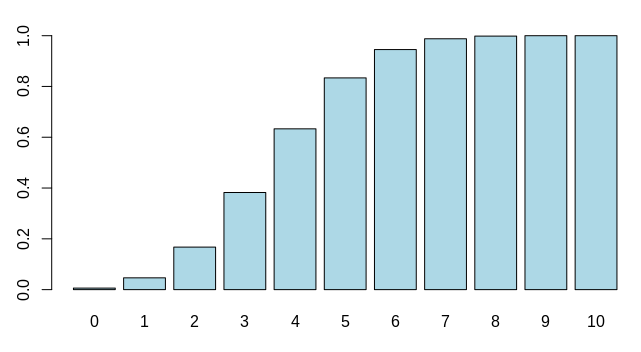
\includegraphics[width=0.99\linewidth]{random_distribution_binomial_2}
      \caption{Binomial c.d.f.}
      \label{fig:bin_cdf}
    \end{minipage}
\end{figure}
% subsubsection properties06 (end)

\subsubsection{Geometric Distribution} % (fold)
\label{ssub:geometric_distribution}

Consider a Bernoulli trial with probability of success $p$, the number of
independent trials that result in \emph{failure} obtained before the first
success follows a Geometric distribution with parameter $p$.
\begin{gather*}
    X \sim \mathcal{G}(p)
    \intertext{with}
    P(X=x) = p(1-p)^x,\;\;\; x \in \{0,1,2,\dots,n\}\\
    \intertext{and have expectation and variance}
    \E[X] = \dfrac{1-p}{p}, \quad V[X] = \dfrac{1-p}{p^2}
\end{gather*}\todo{Add base example that serves as base experiment.} 

Using this base experiment we cant try to fit other rand. exp. and see if this 
distribution is valid.
\begin{figure}[!ht]
    \begin{minipage}{0.45\linewidth}
      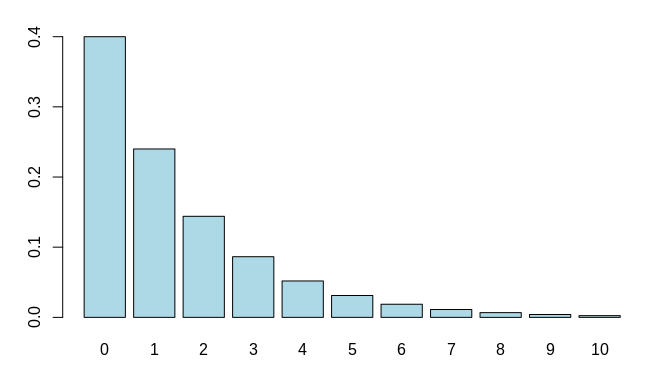
\includegraphics[width=0.99\linewidth]{random_distribution_geometric_1}
      \caption{Geometric p.m.f.}
      \label{fig:gom_pmf}
    \end{minipage}
    \hfill
    \begin{minipage}{0.45\linewidth}
      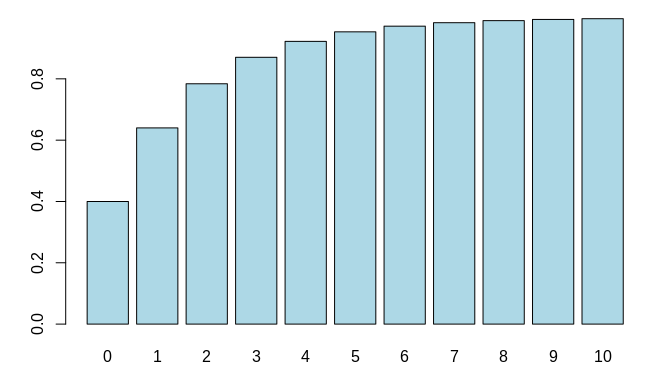
\includegraphics[width=0.99\linewidth]{random_distribution_geometric_2}
      \caption{Geometric c.d.f.}
      \label{fig:geom_cdf}
    \end{minipage}
\end{figure}
% subsubsection geometric_distribution (end)

\subsection{Negative Binomial Distribution} % (fold)
\label{sub:negative_binomial_distribution}

Consider a Bernoulli trial with probability of success $p$, the number of
failures (independent trials that result in failure) before the $k$-th success
(that is, \textbf{number of trials} until $k$-success) follows a Negative
Binomial distribution with parameters $k$ and $p$.
\begin{gather*}
    X \sim NB(k,p)\\
    \intertext{with}
    P(X=x) = \binom{x+k-1}{x} p^k(1-p)^x, \quad x \in \{0,1,2,\dots,n\}\\
    \intertext{and have expectation and variance}
    \E[X] = \dfrac{k(1-p)}{p}, \quad V[X] = \dfrac{k(1-p)}{p^2}
\end{gather*}

\textbf{Note: Be careful with the definition.} This distribution counts the
\textbf{number of fails} not the number of fails $+$ success
\todo{Add base example that serves as base experiment.} Using this base
experiment we cant try to fit other rand. exp. and see if this distribution is
valid.
\begin{figure}[!ht]
    \begin{minipage}{0.45\linewidth}
      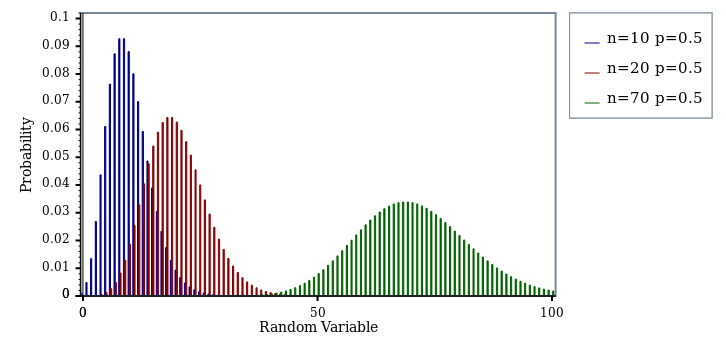
\includegraphics[width=0.99\linewidth]{random_distribution_negbinomial_1}
      \caption{Negative Bin. p.m.f.}
      \label{fig:neg_bin_pmf}
    \end{minipage}
    \hfill
    \begin{minipage}{0.45\linewidth}
      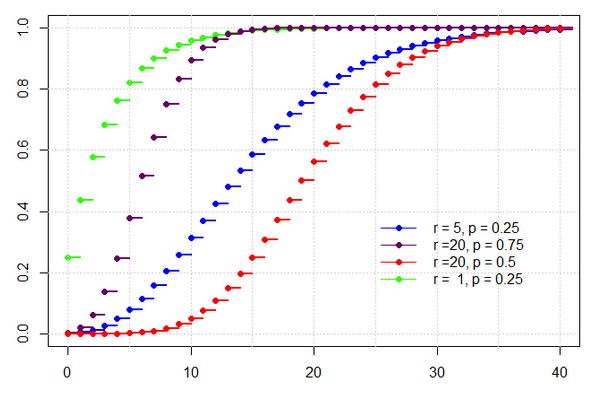
\includegraphics[width=0.99\linewidth]{random_distribution_negbinomial_2}
      \caption{Negative Bin. c.d.f.}
      \label{fig:neg_bin_cdf}
    \end{minipage}
\end{figure}
% subsection negative_binomial_distribution (end)

\subsection{Hypergeometric Distribution} % (fold)
\label{sub:hypergeometric_distribution}

Consider a \textbf{finite population} with $N_1+N_2$ objects, such that $N_1$
are of type 1 and $N_2$ are of type 2. A total number of $k$ objects are
selected from the population \textbf{without replacement}. The number of objects
of type $N_1$ in the selection follows a Hypergeometric distribution with
parameters $N_1, N_2$, and $k$.
\begin{gather*}
    X \sim H(N_1,N_2,k)\\
    \intertext{with}
    P(X=x) = \dfrac{\binom{N_1}{x}\binom{N_2}{k-x}}{\binom{N_1+N_2}{k}}, \quad x
    \in \{\max\{0,k-N_2\},\dots,\min\{k,N_1\} \}\\
    \intertext{and have expectation and variance}
    \E[X] = \dfrac{kN_1}{N_1+N_2}, \quad V[X] =
    k\cdot\dfrac{N_1N_2}{(N_1+N_2)^2}\cdot\dfrac{N_1+N_2-k}{N_1+N_2-1}
\end{gather*}

\todo{Add base example that serves as base experiment.} Using this base
experiment we cant try to fit other rand. exp. and see if this distribution is
valid.
\begin{figure}[!ht]
    \begin{center}
        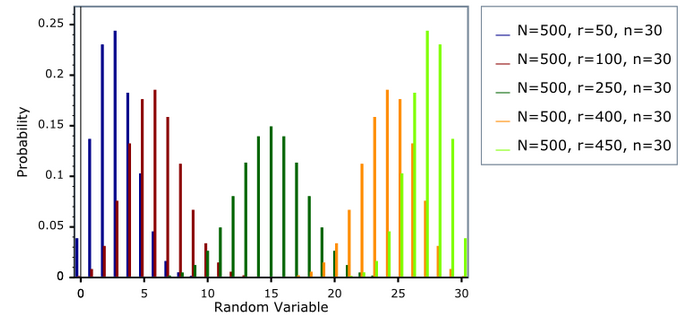
\includegraphics[width=0.99\linewidth]{random_distribution_hyperg_1}
        \caption{Hypergeometric p.m.f.}
        \label{fig:hyp_geom_pmf}
    \end{center}
\end{figure}
% subsection hypergeometric_distribution (end)

\subsection{Poisson Distribution} % (fold)
\label{sub:poisson_distribution}

The number of events that occur in a region of space (or time) independently one
from the others and at a constant rate $\lambda >0$ follows a Poisson
distribution with parameter $\lambda$.
\begin{gather*}
    X \sim \mathcal{P}(\lambda)\\
    \intertext{with}
    P(X=x) = e^{-\lambda}\dfrac{\lambda^x}{x!}, \quad x \in \{0,1,2,\dots,n\}\\
    \intertext{and have expectation and variance}
    \E[X] = \lambda, \quad V[X] = \lambda
\end{gather*}\todo{Add base example that serves as base experiment.} Using this 
base experiment we cant try to fit other rand. exp. and see if this distribution 
is valid.

\subsubsection{Properties} % (fold)
\label{ssub:properties07}

If $X$ and $Y$ are independent, and $X \sim \mathcal{P}(\lambda_1), Y \sim
\mathcal{P}(\lambda_2)$ then 
\begin{equation*}
    X+Y \sim \mathcal{P}(\lambda_1+\lambda_2)
\end{equation*}

\begin{figure}[!ht]
    \begin{minipage}{0.45\linewidth}
      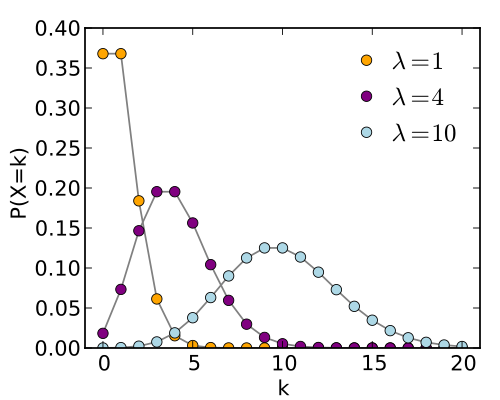
\includegraphics[width=0.99\linewidth]{random_distribution_poisson_1}
      \caption{Poisson p.m.f.}
      \label{fig:psn_pmf}
    \end{minipage}
    \hfill
    \begin{minipage}{0.45\linewidth}
      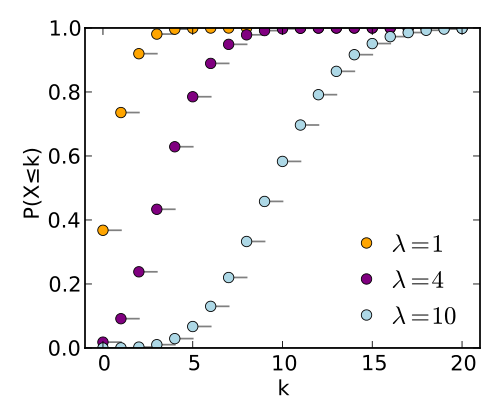
\includegraphics[width=0.99\linewidth]{random_distribution_poisson_2}
      \caption{Poisson c.d.f.}
      \label{fig:psn_cdf}
    \end{minipage}
\end{figure}
% subsubsection properties07 (end)
% subsection poisson_distribution (end)

\subsection{Multi Bernoulli Distribution} % (fold)
\label{sub:multi_bernoulli_distribution}

\todo[inline]{write this}
% subsection multi_bernoulli_distribution (end)

\subsection{Zero Inflated Poisson Distribution} % (fold)
\label{sub:zero_inflated_poisson_distribution}

\todo[inline]{write this}
% subsection zero_inflated_poisson_distribution (end)
% section discrete_random_distributions (end)

\section{Continuous Random Variables} % (fold)
\label{sec:continuous_random_variables}

\todo[inline]{Add moment generating function section}
A continuous r.v. $X$ is the one that satisfies the following conditions:
\begin{itemize}
    \item The distribution function $F_x$ is always continuous.
    \item The distribution function $F_x$ is differentiable and its derivative
    is continuous except for a countable set of points.
\end{itemize}

\subsection{Probability density function} % (fold)
\label{sub:probability_density_function}

The p.d.f. (also referred as density mass function) of $X$ is a function such as
$f_X:\mathbb{R}\rightarrow\mathbb{R}$ and it is 
\begin{equation*}
    f_X(x)=\begin{cases}
          0& \text{if }x\in S\\
    F_X'(x)& \text{if }x\notin S
    \end{cases} 
\end{equation*}

\begin{tcolorbox}
    Note that the above definition is similar to:
    \begin{equation*}
        P(X\in A) = \int_A f_X(x)\,dx
    \end{equation*}
    
    For $A\subset\mathbb{R}$ a borelian set.
\end{tcolorbox}

\missingfigure{explanatory p.d.f.}
% subsection probability_density_function (end)

\subsection{Cumulative distribution function} % (fold)
\label{sub:cumulative_distribution_function}

\begin{equation*}
    F_X(x) = P(X\leq x) = \int_{-\infty}^\infty f_X(t)\,dt
\end{equation*}

\subsubsection{Properties} % (fold)
\label{ssub:properties08}

\begin{itemize}
    \item $\lim_{x\rightarrow-\infty}F(x)=0$
    \item $\lim_{x\rightarrow\infty}F(x)=1$
    \item $F$ is non decreasing
    \item $F$ is continuous
\end{itemize}

\begin{tcolorbox}
    In order to compute the probability that $X$ lies in an interval $[a,b]$
    just
    \begin{equation*}
        P(a\leq X\leq b) = F_X(b)-F_X(a)
    \end{equation*}
\end{tcolorbox}
% subsubsection properties08 (end)

\subsubsection{Relationship between p.d.f and c.d.f.} % (fold)
\label{ssub:relationship_between_p_d_f_and_c_d_f_}

It's important to note that the c.d.f. is just the primitive of the p.d.f. and
thus, the p.d.f. is the derivative of the c.d.f.
\begin{equation*}
    F_X(x)=\int_{-\infty}^x f_X(t)\,dt \quad\text{and} \quad f_X(x) = F_X'(x)
\end{equation*}
% subsubsection relationship_between_p_d_f_and_c_d_f_ (end)
% subsection cumulative_distribution_function (end)

\subsection{Mean, variance and quantiles} % (fold)
\label{sub:mean_variance_and_quantiles}

\subsubsection{Mean} % (fold)
\label{ssub:mean}

\begin{equation*}
    \E[X]  = \int_{-\infty}^\infty xf_X(x)dx
\end{equation*}

The mean holds the same properties as it is does in its discrete form
\begin{itemize}
    \item $\E[aX+b] = a\E[X]+b$
    \item $\E[g(X)] = \int g(x)f_X(x)dx$
    \item $\E[(X-\E[X])^2] = \min_{x\in\mathbb{R}} \mathbb{E}[(X-x)^2]$
\end{itemize}
% subsubsection mean (end)

\subsubsection{Variance} % (fold)
\label{ssub:variance}

\begin{equation*}
    \Var[X]=\E[(X-\E[X])^2] = \int (x-\E[X])^2 f_X(x)\,dx
\end{equation*}
% subsubsection variance (end)

\subsubsection{Properties} % (fold)
\label{ssub:properties09}

\todo[inline]{I took advantage of the \texttt{amsmath} 
feature to create new mathematical operators to create some that I'm seeing that
 are recurrent throughout the text, such as variance.
I have defined it as $Var$ and not $V$, I give it to your consideration, if you 
decide to change it just go to \texttt{line 47} of the \texttt{main.tex} file to
 define it to your liking.}

\begin{itemize}
    \item $\Var[X]\geq 0$
    \item $\Var[X]=\E[X^2]-\E[X]^2$
    \item $\Var[aX+b] = a^2V[X] \quad \forall a,b \in \mathbb{R}$
\end{itemize}
% subsubsection properties09 (end)

\subsubsection{Standard deviation} % (fold)
\label{ssub:standard_deviation}

\begin{equation*}
    \sigma_X = \sqrt{\Var[X]}
\end{equation*}

\todo[inline]{complete section with, median, quantiles}
% subsubsection standard_deviation (end)
% subsection mean_variance_and_quantiles (end)
% section continuous_random_variables (end)

\section{Continuous Random Distributions} % (fold)
\label{sec:continuous_random_distributions}

\subsection{Uniform Distribution} % (fold)
\label{sub:uniform_distribution}

\todo[inline]{write description}

\begin{gather*}
    X \sim U(a,b)\\
    \intertext{with}
    f_X(x)=
    \begin{cases}
        \dfrac{1}{b-a} & \text{if } a\leq x \leq b\\
                      0& \text{otherwise}
    \end{cases}\\
    \intertext{and}
    \E[X]=\dfrac{a+b}{2}, \quad\Var[X]=\dfrac{(b-a)^2}{12}
\end{gather*}

\missingfigure{pdf and cdf}
% subsection uniform_distribution (end)

\subsection{Exponential distribution} % (fold)
\label{sub:exponential_distribution}

Used to measure the time between the occurrence of two events in a Poisson
distribution $X_t\sim\mathcal{P}(t\lambda)$ where $t$ is the number of events in
$[0,t]$.
\todo[inline]{write description}
\begin{gather*}
    T \sim Exp(\lambda)\\
    \intertext{with c.d.f.}
    F_T(t)=
    \begin{cases}
        1-e^{-\lambda t} & \text{if } t\geq 0\\
                        0& \text{if } t<0
    \end{cases}\\
    \intertext{with p.d.f.}
    f_T(t)=
    \begin{cases}
        \lambda e^{-\lambda t} & \text{if } t\geq 0\\
                              0& \text{if } t<0
    \end{cases}\\
    \intertext{and}
    \E[T]=\lambda^{-1}, \quad \Var[T]=\lambda^{-2}
\end{gather*}

\begin{tcolorbox}
    Lack of memory property
    \begin{equation*}
        P(T>t_1 + t_2 |\;T>t_1) = P(T>t_2)
    \end{equation*}
\end{tcolorbox}

\missingfigure{pdf and cdf}
% subsection exponential_distribution (end)

\subsection{Normal Distribution} % (fold)
\label{sub:normal_distribution}

\todo[inline]{write description}

\begin{gather*}
    X \sim \mathcal{N}(\mu,\sigma)\\
    \intertext{with}
    f_X(x)=\dfrac{1}{\sigma\sqrt{2\pi}}\exp\Bigl\{\dfrac{-(x-\mu)^2}{2\sigma^2}
    \Bigr\}, \quad x\in\mathbb{R}
\end{gather*}
if $\mu=0$ and $\sigma=1$ then it is said that $\mathcal{N}$ is in standard
normal and
\begin{equation*}
    f_X(x)=\dfrac{1}{\sqrt{2\pi}}e^{-x^2/2}, \quad x\in\mathbb{R}
\end{equation*}

\begin{tcolorbox}
    Note that a linear transformation of a normal is also a normal
    \begin{equation*}
        aX+b \sim \mathcal{N}(a\mu+b, \quad|a|\sigma)
    \end{equation*}
\end{tcolorbox}

\begin{tcolorbox}
    Probably the most important transformation is the one called
    \textbf{standarization}
    \begin{equation*}
        \dfrac{X-\mu}{\sigma}\sim\mathcal{N}(0,1)
    \end{equation*}
\end{tcolorbox}
\missingfigure{pdf and cdf}

\todo[inline]{COMPLETE WITH gamma, beta distributions}
% subsection normal_distribution (end)
% section continuous_random_distributions (end)

\section{Random Vectors} % (fold)
\label{sec:random_vectors}

Until now the only distributions that we have seen are in $\mathbb{R}$, or in
other words in one single dimension. Now we are going to study random variables
in more dimensions.

\subsection{Marginal distributions} % (fold)
\label{sub:marginal_distributions}


The distributions of each of the components of a r.v. alone is referred to as
Marginal distribution.

 \subsubsection{Random Vector}
 A random vector is a measurable mapping from a sample space $S$ into
 $\mathbb{R}^d$. For example, a bivariate random vector maps $S$ into
 $\mathbb{R}^2$
 \begin{equation*}
     (X,Y):S\rightarrow\mathbb{R}^2
 \end{equation*}

\subsubsection{Joint distribution of a r.v.} % (fold)
\label{ssub:joint_distribution_of_a_r_v_}

The joint distribution is the one that describes the behavior of all variables
that compose the random vector. So, since now, we are going to talk about joint
distributions of two or more random variables.
% subsubsection joint_distribution_of_a_r_v_ (end)
% subsection marginal_distributions (end)

\subsection{Discrete random vectors} % (fold)
\label{sub:discrete_random_vectors}

Let $X, Y$ be two discrete random variables on the same probability space.

\subsubsection{Joint probability mass function} % (fold)
\label{ssub:joint_probability_mass_function}

\begin{gather*}
    p_{X,Y}(x,y)=P(X=x,Y=y)\\
    \intertext{with}
    p_{X,Y}(x,y)>0\\
    \intertext{and}
    \sum_x\sum_yp_{X,Y}(x,y)=1
\end{gather*}
% subsubsection joint_probability_mass_function (end)

\subsubsection{Joint cumulative distribution function} % (fold)
\label{ssub:joint_cumulative_distribution_function}

\begin{equation*}
    \begin{split}
        F_{X,Y}(x_0,y_0)& =P(X\leq x_0,Y\leq y_0)\\
                        &= \sum_{x\leq x_0}\:\sum_{y\leq y_0}p_{X,Y}(x,y)
    \end{split}
\end{equation*}
% subsubsection joint_cumulative_distribution_function (end)

\subsubsection{Marginal discrete distributions} % (fold)
\label{ssub:marginal_discrete_distributions}

Given $X, Y$ with $p_{X,Y}(x,y)$ his joint probability mass function.
\begin{itemize}
    \item \textbf{Marginal p.m.f of X}:
    \begin{equation*}
        p_X(x)=P(X=x)=\sum_yP(X=x,Y=Y)=\sum_yp_{X,Y}(x,y)
    \end{equation*}
    \item \textbf{Marginal p.m.f of Y}:
    \begin{equation*}
        p_Y(y)=P(Y=y)=\sum_xP(X=x,Y=Y)=\sum_xp_{X,Y}(x,y)
    \end{equation*}
\end{itemize}
% subsubsection marginal_discrete_distributions (end)
% subsection discrete_random_vectors (end)

\subsection{Continuous random vectors} % (fold)
\label{sub:continuous_random_vectors}

Let $X, Y$ be two continuous random variables on the same probability space.

\subsubsection{Joint density mass function} % (fold)
\label{ssub:joint_density_mass_function}

\begin{gather*}
    f_{X,Y}(x,y)=P(a\leq X \leq b, c\leq Y \leq d) = \int_{a}^b\int_{c}^df_{X,Y}
    (x,y)\,dydx\\
    \intertext{with}
    f_{X,Y}(x,y)>0\\
    \intertext{and}
    \int_{-\infty}^\infty\int_{-\infty}^\infty f_{X,Y}(x,y)\,dydx=1
\end{gather*}
% subsubsection joint_density_mass_function (end)

\subsubsection{Joint cumulative distribution function} % (fold)
\label{ssub:joint_cumulative_distribution_function}

\begin{equation*}
    F_{X,Y}(x_0,y_0)=P(X\leq x_0,Y\leq y_0) = \int_{-\infty}^{x_0}\int_{-\infty}
    ^{y_0}f_{X,Y}(x,y)\,dydx
\end{equation*}
% subsubsection joint_cumulative_distribution_function (end)

\subsubsection{Marginal continuous distributions} % (fold)
\label{ssub:marginal_continuous_distributions}

Given $X, Y$ with $f_{X,Y}(x,y)$ his joint density mass function.
\begin{description}
    \item[Marginal p.d.f of $X$:]
    \begin{equation*}
        f_X(x)=\int_{-\infty}^\infty f_{X,Y}(x,y)\,dy
    \end{equation*}
    \item[Marginal p.d.f of $Y$:]
    \begin{equation*}
        f_Y(y)=\int_{-\infty}^\infty f_{X,Y}(x,y)\,dx
    \end{equation*}
\end{description}

\todo[inline]{example with image of the diamond distribution}
% subsubsection marginal_continuous_distributions (end)
% subsection continuous_random_vectors (end)

\subsection{Independence of random vectors} % (fold)
\label{sub:independence_of_random_vectors}

$X$ and $Y$ are independent if any of the followings conditions

\begin{multicols}{2}
\setlength{\columnseprule}{0.5pt}
    \textbf{Discrete Variables} 
    \begin{multline*} 
        p{Y|X}(y|x)=p_Y(y)\\
        p_{X|Y}(x|y)=p_X(x)\\
        p_{X,Y}(x,y)=p_X(x)p_Y(y)
    \end{multline*}
    \textbf{Continuous Variables} 
    \begin{multline*}
        f{Y|X}(y|x)=f_Y(y)\\
        f_{X|Y}(x|y)=f_X(x)\\
        f_{X,Y}(x,y)=f_X(x)f_Y(y)
    \end{multline*}
\end{multicols}

\missingfigure{square random vector showing the only true Independence variables}
% subsection independence_of_random_vectors (end)

\subsection{Transformations of random vectors} % (fold)
\label{sub:transformations_of_random_vectors}

Consider a d-variate r.v. $\textbf{X}=(X_1,\dots,X_d)^t$ (notice the bold X) and a
function $g:\mathbb{R}^d \rightarrow \mathbb{R}^k$ then
$\textbf{Y}=g(\textbf{X})$ is a k-variate random vector. Note that if $k=1$ then
$Y=g(\textbf{X})$ is a random variable (notice that the bold Y disappears here).

\subsubsection{Mean of a univariate transformation} % (fold)
\label{ssub:mean_of_a_univariate_transformation}

\begin{itemize}
    \item $\textbf{X}$ discrete:
    \begin{equation*}
         \E[Y]=\E[g(\textbf{X})]=\sum g(\textbf{x})p_\textbf{X}(\textbf{x})
     \end{equation*}
    \item $\textbf{X}$ continuous:
    \begin{equation*}
        \E[Y]=\E[g(\textbf{X})]=\int_{\mathbb{R}^d} g(\textbf{x})f_\textbf{X}
        (\textbf{x})\,d\textbf{x}
    \end{equation*}
\end{itemize}
% subsubsection mean_of_a_univariate_transformation (end)

\subsubsection{Join density mass function of a transformation} % (fold)
\label{ssub:join_density_mass_function_of_a_transformation}

Is the jacobian matrix
\todo[inline]{complete, or maybe remove from here}
% subsubsection join_density_mass_function_of_a_transformation (end)

\subsubsection{Convolutions or sum of independent r.v.} % (fold)
\label{ssub:convolutions_or_sum_of_independent_r_v_}

\todo[inline]{write this}
% subsubsection convolutions_or_sum_of_independent_r_v_ (end)
% subsection transformations_of_random_vectors (end)

\subsection{Mean Vector} % (fold)
\label{sub:mean_vector}

The mean vector of a random vector $\textbf{X}$ is a column vector with
components equals to the mean of the components
\begin{equation*}
    \mu = \E[\textbf{X}] = 
\begin{pmatrix}
    \E[X_1]\\
    \E[X_2]\\
    \vdots\\
    \E[X_d]
\end{pmatrix}
\end{equation*}
% subsection mean_vector (end)

\subsection{Covariance} % (fold)
\label{sub:covariance}

The covariance is a value that measures how one value vary respect the other. Is
one of the principal values used to determine if two variables are independent.
\begin{equation*}
    \Cov[X,Y] = \E[(X-\E[X])(Y-\E[Y])] = \E[XY]-\E[X]\E[Y]
\end{equation*}
% subsection covariance (end)

\subsection{Correlation} % (fold)
\label{sub:correlation}

The correlation is a value that measures the dependency between two variables.

\subsubsection{Pearson's product-moment coefficient} % (fold)
\label{ssub:pearson_s_product_moment_coefficient}

The most popular measure of dependency. It's a value in $[-1,1]$ 
\begin{equation*}
    \rho_{X,Y} = \dfrac{\Cov[X,Y]}{\sqrt{\Var[X]\Var[Y]}}
\end{equation*}

\missingfigure{picture showing the 4 zones of a correlation}

\begin{tcolorbox}
    Notice that, if $X$ and $Y$ are independent then $\Cov[X,Y]=0$ and the
    reverse does not necessary hold. Correlation is not causality.    
\end{tcolorbox}

\todo[inline]{add more types of correlations, linear and not linear, rank-corr etc.}
% subsubsection pearson_s_product_moment_coefficient (end)
% subsection correlation (end)

\subsection{Covariance matrix} % (fold)
\label{sub:covariance_matrix}

Denoted by $\Sigma$ is a square matrix $d \times d$ symmetric positive
semidefinite matrix, such that the element in position $(i,j)$ is
$\Cov[X_i,X_j]$
\todo[inline]{complete}

\subsubsection{Linear transformations} % (fold)
\label{ssub:linear_transformations}

\todo[inline]{complete}
% subsubsection linear_transformations (end)
% subsection covariance_matrix (end)

\subsection{Linear combinations of components of a random vector} % (fold)
\label{sub:linear_combinations_of_components_of_a_random_vector}

\todo[inline]{complete with definition and properties}
% subsection linear_combinations_of_components_of_a_random_vector (end)

\subsection{Multivariate Normal Distribution} % (fold)
\label{sub:multivariate_normal_distribution}

\begin{equation*}
    \textbf{X} \sim \mathcal{N}_d(\mu,\Sigma)
\end{equation*}
    
\todo[inline]{complete}

\missingfigure{descriptive figure with different parameters}
% subsection multivariate_normal_distribution (end)

\subsection{Bivariate Normal distribution} % (fold)
\label{sub:bivariate_normal_distribution}
\begin{gather*}
    (X_1,X_2)^t \sim \mathcal{N}_2(\mu,\Sigma)\\
    \intertext{with}
    \mu=\begin{pmatrix}
    \mu_1\\
    \mu_2
    \end{pmatrix}
    \quad 
    \Sigma=\begin{bmatrix}
    \sigma_1^2 & \rho_{\sigma_1,\sigma_2}\\
    \rho_{\sigma_2,\sigma_1} & \sigma^2_2
    \end{bmatrix}
\end{gather*}

\todo[inline]{complete}

\missingfigure{descriptive figure with different parameters}
% subsection bivariate_normal_distribution (end)

\subsection{Multinomial Distribution} % (fold)
\label{sub:multinomial_distribution}

\begin{equation*}
    \textbf{X} \sim M(n,\textbf{p})
\end{equation*}

\todo[inline]{complete}
\missingfigure{descriptive figure with different parameters}
% subsection multinomial_distribution (end)
% section random_vectors (end)

\section{Mixtures} % (fold)
\label{sec:mixtures}

Let $F_1,F_2,\dots,F_k$ be c.d.f. of different distributions and
$p_1,p_2,\dots,p_k>0$ with $\sum_{i=1}^kp_i=1$, then a new c.d.f. of a mixture
distribution is defined as
\begin{equation*}
    G(x) = p_1F_1(x) + \dots + p_kF_k(x)
\end{equation*}

This new distribution mixes the later distributions according to the probability
 distribution given by $p_1,\dots,p_k$. The c.d.f., density (or probability) 
mass function, or the random number generation can be done directly with the 
original distributions, BUT the quantile function is not straightforwardly 
computed from the ones of the original distributions. \todo{remove this last 
paragraph?}

\missingfigure{mixture of two normals}

\subsection{Mean and variance} % (fold)
\label{sub:mean_and_variance}

If $G=\sum^kp_iF_i$ with mean $\mu$ and variance $\sigma^2$
\begin{align*}
    \mu &= \sum_{i=1}^k p_i\mu_i & \sigma^2 &= \sum_{i=1}^k p_i
    (\mu^2_i+\sigma^2_i)-\mu^2
\end{align*}
% subsection mean_and_variance (end)

\subsection{Uncountable or continuous Mixtures} % (fold)
\label{sub:uncountable_or_continuous_mixtures}

Let $\omega$ be a weight function 
\begin{equation*}
    G(x) = \int_A \omega(a)F_a(x)\,da
\end{equation*}
\todo[inline]{complete this}
% subsection uncountable_or_continuous_mixtures (end)
% section mixtures (end)

\section{Some statistics?} % (fold)
\label{sec:some_statistics_}

\todo[inline]{probably move this to inference chapter}

\subsection{Lorenz curve} % (fold)
\label{sub:lorenz_curve}

If $X\geq 0$ 
\begin{equation*}
    L_X(x) = \dfrac{1}{\E[X]}\int_0^x F^{-1}_X(t)\,dt
\end{equation*}

The Lorenz curve represents the proportion of a given characteristic (wealth) 
earned by the fraction $x$ of individuals with the smallest value in the 
characteristic (poorest individuals). \todo{review this and write about his 
generalized form}

\missingfigure{lorenz curve}
% subsection lorenz_curve (end)

\subsection{Gini coefficient} % (fold)
\label{sub:gini_coefficient}

The Gini index or Gini coefficient equals twice the area between the Lorenz curve
and the line segment from $(0,0)$ to $(1,1)$
\begin{equation*}
    G(X) = 1-2\int_0^1L_X(t)dt = \dfrac{\text{GMD}(X)}{\E[X]}
\end{equation*}

\subsubsection{Gini mean difference}
Let $X,Y$ be independent and follow the same distribution
\begin{equation}
    \text{GMD}(X) = \dfrac{1}{2}\E[|X-Y|]
\end{equation}
% subsection gini_coefficient (end)
% section some_statistics_ (end)
% chapter probability (end)
